% results.tex
\subsection{Integrated Vapor Transport}
We use data from the integrated water vapor transport (\emph{IVT}) model\makenote{needs citation}
  of atmospheric rivers as a means of testing these models.  An atmospheric river is a meteorological
  event of local concentration of water vapor in the atmosphere that moves with wind patterns.
  Understanding extremal dependence in atmospheric rivers, for instance, grants hydrological engineers
  a greater understanding of how and where to build ground water capacity to handle precipitation.
  California suffers persistent, extended droughts--if ground water transportation and holding capacity
  (canals, reservoirs) are not built to manage extreme precipitation without adequate understanding of
  the extremal dependence, then we may not install adequate capacity and thus experience flooding.
  Alternatively, if we install too much capacity everywhere, then we are wasting money that could be
  better spent elsewhere.

Fitting our models to this data requires some pre-processing.  The marginal distributions of the
  IVT data appear naturally log-normal, which falls into the domain of attraction of a Gumbel
  distribution.  Given that, we can apply a high threshold, and exceedances over that threshold can
  be modelled as Generalized Pareto.  Our modelling begins with that assessment.  As estimating
  the Pareto parameters is not yet our focus in this analysis, we choose to apply the threshold
  using the empirical CDF.  That is, for a given $t$, let $b_{tl} = \hat{F}_l^{-1}(1 - t^{-1})$.  For
  this analysis, we set $t = 20$, indicating the marginal $95$ percentile.  The other parameters of the
  generalized Pareto--the scale parameter $\alpha_{tl}$ and the extremal index $\chi_l$--are set via
  maximum likelihood.  A fully Bayesian model formulation will allow their varying within a
  distribution, but such a model formulation will not be conducive to fitting by Markov-chain Monte
  Carlo methods.

After the thresholding and maximum likelihood estimation of the parameters of the Pareto, we scale
  the data to the standard multivariate Pareto.  Dividing each standardized observation by its
  $\mathcal{L}_{\infty}$ norm, we project the standardized data onto $\mathcal{S}_{\infty}^{d-1}$.
  Data in sequence represents observations in time, and these are heavily correlated.  As such, we
  choose to \emph{decluster} the observations, such that, by observing a sequence of observations
  $\bm{ z}$ for which $\inorm{z_i} > 1$ for each observation in sequence, we keep only the observation
  with the greatest observed $\mathcal{L}_{\infty}$ norm.  The complete procedure is outlined in
  Algorithm~\ref{algo:processing}.

\begin{algorithm}
  \label{algo:processing}
  \KwResult{$\bm{ r} : r_i \sim \text{Pareto}(1)$, $\bm{ v} \in \mathcal{S}_{\infty}^{d-1}$}
  \For{$l = 1,ldots,d$}{
    Set $b_{tl} = \hat{F}_l^{-1}\left(1 - \frac{1}{t}\right)$.\\
    With $\bm{ x}_l > b_{tl}$, fit $a_{tl}$, $\chi_l$ via MLE according to generalized Pareto likelihood.\\
    }
  \For{$i = 1,\ldots,n$}{
    Define $z_{il} = \left(1 + \xi_l\frac{x_{il} - b_{t,l}}{a_{t,l}}\right)_{+}^{1/\xi_l}$\\
    Define $r_i = \pnorm{\bm{ z}_i}{\infty}$, $\bm{ V}_i = \frac{\bm{ z}_i}{\pnorm{\bm{ z}_i}{\infty}}$\\
    }
  Subset $\bm{ r},\bm{ v}$ such that $r_i \geq 1$ for all $r_i\in \bm{r}$.\\
  \If{declustering}{
    \For{$i = 1,\ldots,n$}{
      If $r_i \geq 1$ and $r_{i-1} \geq 1$, drop the lesser (and associated $v_i$) from dataset.\\
    }
  }
\end{algorithm}

We have, at our disposal, two datasets from the IVT model.  One records data from 8 grid cells, covering
  generally the coast of California.  The other, with a higher resolution, records data from 47 grid
  cells covering the same area.  We fit our models to both datasets.

\begin{table}[h]
  \label{tab:dev}
  \centering
  
\begin{tabular}{cccccccc}
\toprule
\multicolumn{4}{c}{ } & \multicolumn{2}{c}{dim = 8} & \multicolumn{2}{c}{dim = 46} \\
\cmidrule(l{3pt}r{3pt}){5-6} \cmidrule(l{3pt}r{3pt}){7-8}
Model & Norm & Mix & Prior & PPL & ES & PPL & ES\\
\midrule
Gamma & L1 &  &  & 1.816 & 0.840 & 6.616 & 1.632\\
Gamma & L1 & DP & Gamma & 0.795 & 0.422 & 4.514 & 1.258\\
Gamma & L1 & DP & LogNormal & 0.386 & 0.277 & 2.396 & 0.822\\
Gamma & L1 & M & Gamma & 0.525 & 0.349 & 3.029 & 0.975\\
Gamma & L1 & M & LogNormal & 0.638 & 0.371 & 3.779 & 1.105\\
\addlinespace
Gamma & L2 &  &  & 1.816 & 0.840 & 6.616 & 1.633\\
Gamma & L2 & DP & Gamma & 0.775 & 0.408 & 5.573 & 1.480\\
Gamma & L2 & DP & LogNormal & 0.370 & 0.265 & 2.424 & 0.835\\
Gamma & L2 & M & Gamma & 0.579 & 0.366 & 2.826 & 0.935\\
Gamma & L2 & M & LogNormal & 0.577 & 0.349 & 5.165 & 1.396\\
\addlinespace
Gamma & Linf & DP & Gamma & 0.845 & 0.444 & 6.348 & 1.651\\
Gamma & Linf & DP & LogNormal & 0.384 & 0.278 & 2.376 & 0.823\\
Gamma & Linf & M & Gamma & 0.538 & 0.352 & 3.067 & 0.986\\
Gamma & Linf & M & LogNormal & 0.584 & 0.359 & 3.785 & 1.129\\
Probit Normal &  & DP & Normal & 0.842 & 0.445 & 8.021 & 1.611\\
\addlinespace
Res. Gamma & L1 &  &  & 1.820 & 0.818 & 6.774 & 1.546\\
Res. Gamma & L1 & DP & Gamma & 0.200 & 0.173 & 2.427 & 0.834\\
Res. Gamma & L1 & DP & LogNormal & 0.230 & 0.193 & 1.642 & 0.656\\
Res. Gamma & L1 & M & Gamma & 0.214 & 0.190 & 1.411 & 0.620\\
Res. Gamma & L1 & M & LogNormal & 0.222 & 0.191 & 1.445 & 0.616\\
\addlinespace
Res. Gamma & L2 &  &  & 1.820 & 0.819 & 6.777 & 1.546\\
Res. Gamma & L2 & DP & Gamma & 0.202 & 0.176 & 2.037 & 0.772\\
Res. Gamma & L2 & DP & LogNormal & 0.273 & 0.210 & 1.652 & 0.643\\
Res. Gamma & L2 & M & Gamma & 0.217 & 0.189 & 1.794 & 0.704\\
Res. Gamma & L2 & M & LogNormal & 0.248 & 0.201 & 1.270 & 0.528\\
\addlinespace
Res. Gamma & Linf & DP & Gamma & 0.191 & 0.168 & 2.019 & 0.776\\
Res. Gamma & Linf & DP & LogNormal & 0.228 & 0.191 & 1.458 & 0.589\\
Res. Gamma & Linf & M & Gamma & 0.219 & 0.191 & 1.554 & 0.664\\
Res. Gamma & Linf & M & LogNormal & 0.222 & 0.189 & 1.266 & 0.530\\
\bottomrule
\end{tabular}

  \caption{Model comparison metrics: Posterior Predictive Loss and Energy Score criteria from fitted
    models against the IVT data.  All presented models are DP mixtures; the \emph{Model} field
    identifies the kernel distribution.  For both criteria, lower is better.}
\end{table}

In Table~\ref{tab:dev} we see the same model preference towards the projected restricted gamma models
  that we saw in Figures~\ref{fig:simes,fig:simppl}.  The unrestricted gamma model is penalized much
  more strongly on real data than we saw with our simulation, performing comparably to the probit-normal
  model.  We also see the restricted gamma model with the log-normal prior performing significantly
  better than the restricted gamma model with the gamma prior on the higher dimensional data, a reversal
  of what we saw on the low dimensional data and indeed from what we saw in the simulation study.

That said, there is much we can glean from this table.  The probit-normal model, developed on a mapping
  from $\mathcal{S}_{2}^{d-1}$ to $(-\infty,\infty)^{d-1}$ via probit transformation of spherical coordinates
  was not competitive with the gamma models on real data, similar to what we saw in the simulation study.

We should also note that we did conduct inference on projected gamma models established on
  $\mathcal{S}_{1}^{d-1}$ and $\mathcal{S}_2^{d-1}$.  Posterior predictive loss and energy score criteria
  favored the model established on $\mathcal{S}_{\infty}^{d-1}$.  We also established finite mixture
  models for all presented distributions, but after tuning the number of mixture components, their
  model performance was, and could only be \emph{as good} as the DP mixture.

\begin{figure}[h]
  \centering
  \label{fig:knnkl}
  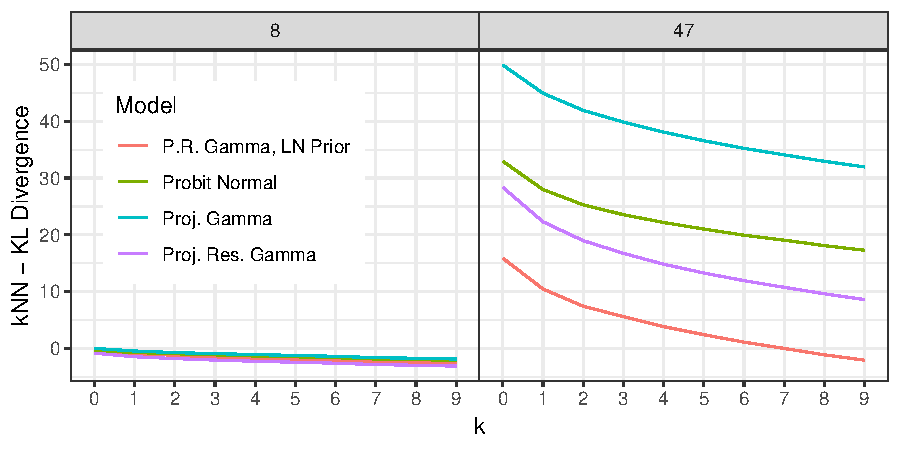
\includegraphics[width = 6in, height = 3in]{./images/knn_kl_divergence_curves}
  \caption{KL Divergence Curves calculated through the KNN-KL Metric, evaluated between the empirical
  dataset and posterior predictive datasets of various models.  The top row corresponds to the
  8-dimensional data, while the bottom row the 47.  All presented models use a Dirichlet process
  prior, the nominal model being the kernel distribution.}
\end{figure}

Interpreting the KL divergence curves in Figure~\ref{fig:knnkl} is more difficult.  As we saw in the
  simulated case in Figure~\ref{fig:simkld}, the general logic of \emph{best} being that which is
  closest to zero is not necessarily in use here.  We interpret a positive value in the KL divergence metric
  as indicating that, for a given point in the given distribution, we must travel \emph{farther} on
  the target distribution to reach the $k$th neighbor as compared to the given distribution.  In this
  regard, we should regard \emph{large} positive values as indicating a particularly poor fit.  In this
  regard, the projected gamma and probit-normal models do not appear to scale well as they performed
  very poorly on the high dimensional data.  For the projected restricted gamma model, the log-normal
  prior appears to scale better than the gamma prior.  This is in keeping with what we observed in
  Table~\ref{table_dev}, but is a different result than what we observed in the simulation study, where
  we observed that the log-normal prior only tended towards the gamma prior, never performing better.

% EOF
